% Provenance (never printed): see sources/outline_sources.md (Year 3:
% geophysical fluid dynamics: rotating-frame equations, Rossby number,
% hydrostatic and geostrophic balance, thermal wind, buoyancy frequency).
% Brief: sources/book5/BRIEFS.md, ch. 19. Curves from
% figdata/bachelor-3/inertial_oscillation.py, thermal_wind.py and
% buoyancy_frequency.py. Exercise and problem values in the Book 5 scratch
% calculator calc/ch19.py. The Steppe of Orrin, its lake, its stations and
% its winds are invented.
\chapter{地球流体动力学}\label{ch:b3:gfd-foundations}

搅动一杯茶，一分钟内漩涡即消失；茶叶聚集在
杯底中央，别的什么也不会发生。海洋和大气
同样受太阳与风的搅动，但它们位于自转的行星上，并且处于
密度不同的分层之中。自转与层结使它们遵循
茶杯里从不显现的规律：风沿等压线吹，而不是
垂直穿过；流体柱拒绝倾斜；对流层上部的风
则写在其下方的温度之中。本章建立
这些大尺度、慢速、薄层流动的方程，以及
决定哪些项重要的少数几个数。

\begin{recall}
旋转坐标系中的科里奥利力与离心力、纳维–斯托克斯
方程和连续性方程、动力黏度、雷诺数和静力
关系均见于物理教材。科里奥利参数 $f = 2\Omega
\sin\varphi$、气压梯度力、地转平衡、
地转风、\omterm{def:b3:gfd-foundations:gradient}{梯度风}和急流，见于本科一年级分册，
其中关于大气环流的一章；
埃克曼层见于其中关于海洋环流的一章；位温、
静力稳定度以及被抬升气块的振荡，都见于
其中关于大气与海洋结构的一章。
\end{recall}

\section{旋转坐标系中的方程}\label{sec:b3:gfd-foundations:equations}

在随地球转动、角速度为
$\vec\Omega$ 的旋转坐标系中，速度为 $\vec u$ 的流体微团满足
\[
\frac{\mathrm D\vec u}{\mathrm Dt} + 2\vec\Omega\times\vec u =
-\frac{1}{\rho}\nabla p + \vec g + \nu\nabla^2\vec u ,
\qquad
\frac{\partial\rho}{\partial t} + \nabla\cdot(\rho\vec u) = 0 ,
\]
其中 $\mathrm D/\mathrm Dt = \partial/\partial t + \vec u\cdot\nabla$ 为
沿微团的导数，$\nu$ 为运动黏度。
离心力已并入万有引力中，二者之和 $\vec g$ 即
有效重力，它与\omterm{def:b3:gravity-geodesy:geopotential}{位势}的等位面垂直，
竖直方向由它定义。自转的影响中只剩科里奥利项 $-2\vec\Omega\times
\vec u$，它不做功，只使微团转向而不改变其速率。
地球的自转角速度为 $\Omega =
\qty{7.292115e-5}{rad/s}$，即一个恒星日为 \qty{23.9345}{h}。
% ledger: geod5:grs80-defining, earth:Trot

对于远小于地球半径 $a$ 的运动，
取局地笛卡儿坐标系即可：$x$ 向东，$y$ 向北，$z$ 向上，
位于纬度 $\varphi$ 处，即下图所示的切平面。此处
$\vec\Omega = \Omega\,(0, \cos\varphi, \sin\varphi)$，动量方程的三个
分量为
\[
\begin{aligned}
\frac{\mathrm Du}{\mathrm Dt} - f v + \tilde f w &= -\frac{1}{\rho}\frac{\partial p}{\partial x} + F_x ,\\
\frac{\mathrm Dv}{\mathrm Dt} + f u &= -\frac{1}{\rho}\frac{\partial p}{\partial y} + F_y ,\\
\frac{\mathrm Dw}{\mathrm Dt} - \tilde f u &= -\frac{1}{\rho}\frac{\partial p}{\partial z} - g + F_z ,
\end{aligned}
\qquad f = 2\Omega\sin\varphi,\quad \tilde f = 2\Omega\cos\varphi ,
\]
其中 $\vec F$ 为摩擦力。对于薄层、近水平的
海洋与大气流动，含 $\tilde f$ 的项被略去：$\tilde f w$
比 $fv$ 小得多，因为 $w \ll v$，而 $\tilde f u$ 仅为
$g$ 的万分之一（见\cref{exo:b3:gfd-foundations:5}）。科里奥利力于是只
在水平方向起作用，通过自转的局地竖直分量
$\Omega\sin\varphi$。

\begin{definition}[$f$ 平面与 $\beta$ 平面]\label{def:b3:gfd-foundations:planes}
在参考纬度 $\varphi_0$ 附近，\emph{$f$ 平面}\index{$f$ 平面}
近似取科里奥利参数为常数，$f = f_0 =
2\Omega\sin\varphi_0$。\emph{$\beta$ 平面}\index{$\beta$ 平面}
近似保留其随向北距离 $y$ 的一阶变化：
$f = f_0 + \beta y$，其中 $\beta = \mathrm df/\mathrm dy = 2\Omega
\cos\varphi_0/a$。
\end{definition}

在 \ang{45} 处，取平均半径 $a = \qty{6371}{km}$，$f_0 =
\qty{1.031e-4}{s^{-1}}$，$\beta = \qty{1.62e-11}{m^{-1}.s^{-1}}$，在
\qty{1000}{km} 的纬度范围内 $f$ 变化了 \qty{16}{\percent}。$f$ 平面
适用于远小于此的运动；$\beta$ 平面则
需用于盆地尺度的洋流和行星波。
% ledger: earth:Rmean, geod5:grs80-defining (values in figdata/bachelor-3/inertial_oscillation.py)

\begin{omfigure}
\begin{minipage}[c]{0.42\linewidth}\centering
\begin{tikzpicture}[>=stealth, font=\small]
\draw[thick] (0,0) circle (2);
\draw[black!40, dashed] (-2,0) -- (2,0);
\draw[->, thick] (0,-2.4) -- (0,2.75) node[above] {$\vec\Omega$};
\draw (0,0) -- (30:2) coordinate (P);
\draw (0.6,0) arc (0:30:0.6);
\node at (15:0.9) {$\varphi$};
\draw[black!60] ($(P)+(120:-1.1)$) -- ($(P)+(120:1.3)$);
\draw[->, omThm, thick] (P) -- ++(0,1.6) node[right] {$\vec\Omega$};
\draw[->, omDef, thick] (P) -- ++(30:0.8) node[anchor=south west, align=left, inner sep=1pt] {$\Omega\sin\varphi$，\\ 向上};
\draw[->, omMeth, thick] (P) -- ++(120:1.386) node[anchor=south, align=center, inner sep=1pt] {$\Omega\cos\varphi$，\\ 向北};
\draw[black!50, densely dotted] ($(P)+(30:0.8)$) -- ($(P)+(0,1.6)$) -- ($(P)+(120:1.386)$);
\draw (P) circle (0.09); \draw ($(P)+(-0.064,-0.064)$) -- ($(P)+(0.064,0.064)$);
\draw ($(P)+(-0.064,0.064)$) -- ($(P)+(0.064,-0.064)$);
\node[font=\scriptsize, anchor=west] at ($(P)+(0.14,-0.03)$) {$x$，东};
\node[font=\scriptsize, black!60] at (-1.15,-0.25) {赤道};
\end{tikzpicture}
\end{minipage}\hfill
\begin{minipage}[c]{0.55\linewidth}\centering
\begin{tikzpicture}
\begin{axis}[width=\linewidth, height=0.72\linewidth, xmin=0, xmax=90, ymin=0, ymax=1.8,
  xlabel={纬度 (\unit{\degree})}, ylabel={$f$ ($10^{-4}$\,\unit{s^{-1}})},
  xtick={0,15,30,45,60,75,90}, tick label style={font=\scriptsize}, label style={font=\small},
  legend style={font=\scriptsize, draw=none, fill=none}, legend pos=north west]
% computed in figdata/bachelor-3/inertial_oscillation.py
\addplot[omDef, thick] table[x=lat, y=f] {figdata/out/bachelor-3-inertial_oscillation-fbeta.dat};
\addplot[omThm, densely dashed] table[x=lat, y=fb] {figdata/out/bachelor-3-inertial_oscillation-fbeta.dat};
\addplot[only marks, mark=*, mark size=1.6pt] coordinates {(45,1.03126)};
\legend{$2\Omega\sin\varphi$, $\beta$ 平面在 \ang{45}}
\end{axis}
\end{tikzpicture}
\end{minipage}

\par\smallskip{\small 左图为纬度 $\varphi$ 处的局地坐标系：$z$
沿局地竖直方向，$y$ 在切平面内指向北方，$x$ 向东，
指向纸面内。旋转矢量分解为绕竖直方向的 $\Omega\sin\varphi$，
它使水平运动发生偏转；绕指北轴的 $\Omega\cos\varphi$，
对薄层流动可略去。右图为科里奥利参数及其
在 \ang{45} 处的 $\beta$ 平面近似：在一段纬度带内近似良好，
远离该带则在赤道与极地附近偏离较大。}\label{fig:b3:gfd-foundations:frame}
\end{omfigure}
% ledger: geod5:grs80-defining, earth:Rmean

另有两个近似可以简化方程，同时不丢失
主要物理内容。第一个涉及密度。

\begin{definition}[布西内斯克近似]\label{def:b3:gfd-foundations:boussinesq}
\emph{布西内斯克近似}\index{布西内斯克近似}将密度写为
$\rho = \rho_0 + \rho'$，其中 $\rho_0$ 为常数，且
$|\rho'| \ll \rho_0$，并保留 $\rho'$，但仅限于与 $g$ 相乘的项。
连续性方程化为 $\nabla\cdot\vec u = 0$，
动量方程为
\[
\frac{\mathrm D\vec u}{\mathrm Dt} + f\,\vec k\times\vec u =
-\frac{1}{\rho_0}\nabla p' + b\,\vec k + \nu\nabla^2\vec u ,
\qquad b = -g\,\frac{\rho'}{\rho_0} ,
\]
其中 $p'$ 为压强与
密度为 $\rho_0$ 的静力压强之差，$\vec k$ 为
竖直向上的单位矢量，$b$ 为浮力。
\end{definition}

在海洋中，$\rho'$ 约为几 \unit{kg/m^3}，相对 \num{1025} 仅占
百分之几，近似非常好。在大气中，密度
约在 \qty{8.5}{km} 高度内降为原来的 $e$ 分之一；近似对
远薄于此的层结成立；更深的流动须将 $\rho_0$ 换为
平均廓线 $\rho_0(z)$，物理内容相同。
% ledger: earth:Hscale

第二个涉及竖直方向。静止流体处于静力
平衡；运动流体只要运动的水平尺度远大于深度，
便可以很好地近似保持这一平衡。

\begin{definition}[静力近似]\label{def:b3:gfd-foundations:hydrostatic}
\emph{静力近似}\index{静力近似}
以静力关系代替运动流体的竖直动量方程，即
$\partial p/\partial z = -\rho g$。
\end{definition}

\begin{proposition}[静力近似成立的条件]\label{prop:b3:gfd-foundations:hydrostatic}
对于水平尺度为 $L$、深度为 $H$、速度为 $U$ 的运动，
若\omterm{def:b3:gfd-foundations:numbers}{罗斯贝数} $U/(fL)$ 至多为一个量级，则竖直加速度
比压强扰动的竖直梯度小一个因子，
该因子的量级为 $(U/fL)\,(H/L)^2$。
\end{proposition}

\begin{proof}
当科里奥利力至少与加速度同量级时，
水平动量方程使水平压强梯度与之平衡：
$p'/(\rho_0 L) \sim fU$，故 $p'/\rho_0 \sim fUL$，
竖直梯度为 $p'/(\rho_0 H) \sim fUL/H$。由连续性方程 $\partial w/\partial z
= -(\partial u/\partial x + \partial v/\partial y)$，可得竖直速度的
量级 $W \sim UH/L$，竖直加速度的量级为
$\mathrm Dw/\mathrm Dt \sim UW/L = U^2H/L^2$。二者之比为 $(U^2H/L^2)/(fUL/H)
= (U/fL)(H/L)^2$。
\end{proof}

水平尺度为 \qty{1000}{km}、对流层深 \qty{10}{km} 的天气系统，
有 $(H/L)^2 = 10^{-4}$，\omterm{def:b3:gfd-foundations:numbers}{罗斯贝数}约为 0.1，
则\omterm{def:b3:gfd-foundations:hydrostatic}{静力近似}的误差量级为 $10^{-5}$。只有在狭窄而深厚的运动中，它才会失效，
例如雷暴的上升气流、海洋中的对流羽流。

\section{旋转流动的尺度}\label{sec:b3:gfd-foundations:scales}

动量方程中哪些项重要，由两个比值决定。

\begin{definition}[罗斯贝数与埃克曼数]\label{def:b3:gfd-foundations:numbers}
对于速度为 $U$、水平尺度为 $L$、深度为 $H$ 的流动，
其所在行星的科里奥利参数为 $f$，\emph{罗斯贝数}\index{罗斯贝数}为
$\mathrm{Ro} = U/(fL)$，即量级为 $U^2/L$ 的加速度
与量级为 $fU$ 的科里奥利力之比。\emph{埃克曼
数}\index{埃克曼数}为 $\mathrm{Ek} = \nu/(fH^2)$，
即量级为 $\nu U/H^2$ 的黏性力与科里奥利力之比；
在湍流中，$\nu$ 由涡黏性代替。
\end{definition}

一个浴缸以 \qty{0.1}{m/s} 的速度在 \qty{0.3}{m} 范围内排水，其\omterm{def:b3:gfd-foundations:numbers}{罗斯贝数}为
数千：地球自转并不决定其
漩涡的旋转方向。一个宽 \qty{1000}{km} 的低压，风速为 \qty{15}{m/s}，其\omterm{def:b3:gfd-foundations:numbers}{罗斯贝数}为
$\mathrm{Ro} \approx 0.14$，而海洋环流的 $\mathrm{Ro} \sim 10^{-4}$。
黏性更弱：水的分子黏度为
\qty{e-6}{m^2/s}，而代表海洋湍流的涡黏度
在竖直方向为 \qtyrange{e-5}{e-3}{m^2/s}，
对于 \qty{1000}{m} 的深度，给出 $\mathrm{Ek} \sim 10^{-5}$。两个数
与雷诺数的关系为 $\mathrm{Re} = UL/\nu =
(\mathrm{Ro}/\mathrm{Ek})(L/H)^2$.
% ledger: stewart:eddy (problem values in calc/ch19.py)

当两个数都很小时，定常水平动量方程只保留
科里奥利力与气压梯度力：流动处于
地转平衡，$f\,\vec k\times\vec u_g = -(1/\rho)\nabla_h p$，这正是
本科一年级分册中从天气图读出的关系。地转是
$\mathrm{Ro}, \mathrm{Ek}\to 0$ 的极限；其修正量级为
$\mathrm{Ro}$，摩擦只作用于相对厚度为
$\sqrt{\mathrm{Ek}}$ 的薄层，即大气底部以及
海洋顶部和底部的埃克曼层。在 $f$ 平面上，地转速度
没有水平散度：$\partial u_g/\partial x + \partial
v_g/\partial y = -(1/\rho f)(\partial^2 p/\partial x\partial y -
\partial^2 p/\partial y\partial x) = 0$，此处 $\rho$ 为常数。

与之相反的极限是没有压强梯度的旋转，
它是旋转流体所能做的最简单的运动。

\begin{definition}[惯性振荡]\label{def:b3:gfd-foundations:inertial}
称\emph{惯性振荡}\index{惯性振荡}为流体的
水平运动，其上除科里奥利力外不受水平力
作用。
\end{definition}

\begin{theorem}[惯性圆]\label{thm:b3:gfd-foundations:inertial}
在 $f$ 平面上，一个以速度 $U$ 运动的流体块，除科里奥利力外不受水平力，
则其速度大小保持不变，并描出半径为
$U/|f|$ 的圆，北半球顺时针、
南半球逆时针，惯性周期为 $2\pi/|f|$，即半个恒星日
除以 $\sin\varphi$。
\end{theorem}

\begin{proof}
方程为 $\mathrm du/\mathrm dt = fv$，$\mathrm dv/\mathrm dt =
-fu$。取 $w = u + \mathrm iv$，则 $\mathrm dw/\mathrm dt = -\mathrm
if\,w$，于是 $w = U\,\mathrm e^{-\mathrm ift}$，对应向东的初速度：
速率 $|w| = U$ 不变，速度方向以角速率 $f$ 转动，
当 $f > 0$ 时顺时针。积分可得位置 $x + \mathrm iy =
(\mathrm iU/f)(\mathrm e^{-\mathrm ift} - 1)$ 绕点
$-\mathrm iU/f$ 作圆周运动，半径为 $U/|f|$。周期为 $2\pi/|f| =
2\pi/(2\Omega|\sin\varphi|)$，而 $2\pi/\Omega$ 即为恒星日。
\end{proof}

在 \ang{45} 处，惯性周期为 \qty{16.9}{h}；流速为
\qty{0.2}{m/s} 的水流沿半径为 \qty{1.94}{km} 的圆周运动。在 \ang{30} 处
周期恰为一个恒星日，而在赤道则没有惯性圆。
风暴使海洋表层运动后随之平息，
海水正是如此运动。北太平洋中，深度为 \qty{15}{m} 的带锚漂流浮标在
1987 年 10 月风暴之后数日内描出回环，并随
平均洋流漂移。下图中的第三条路径，位于圆与
螺线之后。
% ledger: stewart:inertial, earth:Trot (values in figdata/bachelor-3/inertial_oscillation.py)

\begin{omfigure}
\begin{tikzpicture}
\begin{axis}[width=\linewidth, axis equal image, xmin=-3, xmax=18.5, ymin=-4.6, ymax=1.2,
  xlabel={向东距离 (km)}, ylabel={向北距离 (km)},
  tick label style={font=\scriptsize}, label style={font=\small},
  legend style={font=\scriptsize, draw=none, fill=white, fill opacity=0.85, text opacity=1},
  legend pos=south east, legend columns=3]
% computed in figdata/bachelor-3/inertial_oscillation.py
\addplot[black!45, line width=1.6pt] table[x=x, y=y] {figdata/out/bachelor-3-inertial_oscillation-circle.dat};
\addplot[omDef, thick] table[x=x, y=y] {figdata/out/bachelor-3-inertial_oscillation-spiral.dat};
\addplot[omThm, thick] table[x=x, y=y] {figdata/out/bachelor-3-inertial_oscillation-loops.dat};
\addplot[only marks, mark=*, mark size=1.8pt] coordinates {(0,0)};
\legend{无摩擦, 有摩擦, 摩擦与洋流}
\end{axis}
\end{tikzpicture}

\par\smallskip{\small 流体块在四天内的路径。起始时
向东以 \qty{0.2}{m/s} 运动，位于北纬 \ang{45}（圆点处），除科里奥利力外不受其他力：
形成半径为 \qty{1.94}{km} 的圆，每
\qty{16.9}{h} 沿顺时针运行一周（灰色）；若有摩擦使速率
在 \num{2.8}~天内减半，形成向内的螺线（蓝色）；同一流体块受稳定
向东洋流 \qty{0.05}{m/s} 携带，形成一串
逐渐缩小的回环（红色）。}\label{fig:b3:gfd-foundations:inertial}
\end{omfigure}
% ledger: stewart:inertial

地转与惯性圆之间的，是绕高压或低压中心的流动，
此处等压线弯曲，指向中心的加速度
不可再忽略。

\begin{definition}[梯度风]\label{def:b3:gfd-foundations:gradient}
称\emph{梯度风}\index{梯度风}为沿弯曲等压线的
定常、无摩擦流动，其中
气压梯度力、科里奥利力与向心加速度相互平衡。
\end{definition}

\begin{proposition}[曲率修正]\label{prop:b3:gfd-foundations:gradient}
设北半球等压线为半径 $r$ 的圆，
$V_g$ 为其气压梯度所对应的地转速度，记
$\mathrm{Ro}_g = V_g/(fr)$。绕低压中心时，\omterm{def:b3:gfd-foundations:gradient}{梯度风}为
$V = 2V_g/(1 + \sqrt{1 + 4\mathrm{Ro}_g})$，慢于 $V_g$；
绕高压中心时，$V = 2V_g/(1 + \sqrt{1 - 4\mathrm{Ro}_g})$，比地转速度快，且仅当
$\mathrm{Ro}_g \le 1/4$ 时存在。近似到一阶，$V = V_g(1 \mp \mathrm{Ro}_g)$。
\end{proposition}

\begin{proof}
绕低压时风向逆时针旋转；气压梯度力
$fV_g$ 指向中心，科里奥利力 $fV$ 指向外，二者之
差提供向心加速度：$fV_g - fV = V^2/r$。
方程 $V^2 + frV - frV_g = 0$ 的正根为 $V = (fr/2)(\sqrt{1 +
4\mathrm{Ro}_g} - 1)$。上下同乘 $(\sqrt{1 + 4\mathrm{Ro}_g} +
1)/(\sqrt{1 + 4\mathrm{Ro}_g} + 1)$，即得所给公式。绕高压时
风向顺时针旋转，科里奥利力指向内侧：$fV - fV_g =
V^2/r$，故 $V^2 - frV + frV_g = 0$，它仅当 $f^2r^2
\ge 4frV_g$ 时有实根；趋于 $V_g$ 的根在 $\mathrm{Ro}_g \to 0$ 时为
$V = (fr/2)(1 - \sqrt{1 - 4\mathrm{Ro}_g})$。将根式展开，
$V = V_g(1 \mp \mathrm{Ro}_g + \dots)$。
\end{proof}

等压线的\omterm{def:b3:gfd-foundations:numbers}{罗斯贝数}度量了这一修正，对中等尺度的低压，
约为十分之一。条件 $\mathrm{Ro}_g \le 1/4$ 解释了为何
反气旋中心的气压梯度较弱、风较轻，而
低压中心则可能出现陡峭的梯度和大风。

\section{无层结的旋转}\label{sec:b3:gfd-foundations:taylor}

密度均匀的旋转流体，在缓慢运动时，其表现如同
由与旋转轴平行的刚性柱体构成。

\begin{theorem}[泰勒–普劳德曼]\label{thm:b3:gfd-foundations:taylor-proudman}
对于均匀密度、无黏流体的定常流动，若其以
$\vec\Omega$ 旋转、\omterm{def:b3:gfd-foundations:numbers}{罗斯贝数}很小，则速度
沿旋转轴方向不发生变化：$(\vec\Omega\cdot\nabla)\vec u = 0$。
\end{theorem}
\index{泰勒–普劳德曼定理}

\begin{proof}
当 $\mathrm{Ro}\to 0$、流动定常且无黏时，动量方程化为
$2\vec\Omega\times\vec u = -\nabla(p/\rho_0 + \Phi)$，其中 $\Phi$ 为
\omterm{def:b3:gravity-geodesy:geopotential}{位势}。梯度的旋度为零，故 $\nabla\times(\vec\Omega
\times\vec u) = 0$。当 $\vec\Omega$ 为常矢量时，该旋度为 $\vec\Omega
(\nabla\cdot\vec u) - (\vec\Omega\cdot\nabla)\vec u$，而对均匀密度流体有 $\nabla\cdot\vec u
= 0$。
\end{proof}

设 $\vec\Omega$ 沿 $z$ 方向，则 $\partial\vec u/\partial z = 0$：三个
速度分量在每一高度上都相同。若刚性底面在此处禁止
$w$，则处处 $w = 0$，水平流动在各
层都一样。因此，旋转水槽底部的障碍物，其影响
可以一直传到表面：障碍物上方的流体无法越过它，因为
那样会拉伸或压缩柱体，而只能在每一高度绕过它。
留在障碍物上方的那柱流体，称为\emph{泰勒
柱}\index{泰勒柱}。

\begin{omfigure}
\begin{tikzpicture}[>=stealth, font=\small]
% side view
\fill[omDef!8] (0,0) rectangle (5.4,3);
\fill[black!10] (2.1,0) rectangle (3.3,3);
\draw[thick] (0,3.3) -- (0,0) -- (5.4,0) -- (5.4,3.3);
\draw[black!50] (0,3) -- (5.4,3);
\draw[fill=black!45] (2.1,0) .. controls (2.4,0.55) and (3.0,0.55) .. (3.3,0) -- cycle;
\draw[black!60, densely dashed] (2.1,0) -- (2.1,3) (3.3,0) -- (3.3,3);
\foreach \y in {0.8,1.6,2.4} {\draw[->, omDef, thick] (0.3,\y) -- (1.9,\y);
  \draw[->, omDef, thick] (3.5,\y) -- (5.1,\y);}
\draw[->, thick, omThm] (2.7,3.25) -- (2.7,4.0) node[right] {$\vec\Omega$};
\node[font=\scriptsize, align=center] at (2.7,1.7) {泰勒 \\柱};
\node[font=\scriptsize, anchor=north] at (2.7,-0.05) {障碍物};
\node[font=\small] at (2.7,-0.6) {(a) 侧视图};
% top view
\begin{scope}[xshift=6.4cm]
\fill[omDef!8] (0,0) rectangle (5.4,3);
\draw[thick] (0,0) rectangle (5.4,3);
\fill[black!10] (2.7,1.5) circle (0.5);
\draw[black!60, densely dashed] (2.7,1.5) circle (0.5);
\foreach \d/\h in {0.3/0.10, 0.75/0.35, 1.2/0.58} {
  \draw[->, omDef, thick] (0.2,1.5+\d) .. controls (1.6,1.5+\d) and (2.0,1.5+\h+0.62) .. (2.7,1.5+\h+0.62)
     .. controls (3.4,1.5+\h+0.62) and (3.8,1.5+\d) .. (5.2,1.5+\d);
  \draw[->, omDef, thick] (0.2,1.5-\d) .. controls (1.6,1.5-\d) and (2.0,1.5-\h-0.62) .. (2.7,1.5-\h-0.62)
     .. controls (3.4,1.5-\h-0.62) and (3.8,1.5-\d) .. (5.2,1.5-\d);}
\node[font=\small] at (2.7,-0.6) {(b) 从上方看，任一高度};
\end{scope}
\end{tikzpicture}

\par\smallskip{\small \omterm{thm:b3:gfd-foundations:taylor-proudman}{泰勒柱}（示意图）。(a) 在一个装有均匀水并快速旋转的水槽中，
缓慢的流动遇到底部的一个低矮障碍物；障碍物上方的流体（灰色）
被固定在原处直至表面，
各高度的流动都绕着该柱流过，仿佛
障碍物一直延伸到顶部。(b) 从上方看，
各层的流动相同。}\label{fig:b3:gfd-foundations:taylor}
\end{omfigure}

大气和海洋具有层结，而层结会放松这一约束：
层结流体可以随高度变化，变化的方式
由\omterm{thm:b3:gfd-foundations:thermal-wind}{热成风}定理规定。

\section{层结与热成风}\label{sec:b3:gfd-foundations:stratification}

本科一年级分册中曾让稳定大气中的一个气块上升，
发现它在原高度附近振荡。同样的结论对任何层结流体都成立，
而振荡频率正是层结程度的度量。

\begin{definition}[浮力频率]\label{def:b3:gfd-foundations:buoyancy}
静止流体的\emph{浮力频率}\index{浮力频率} $N$ 由
下式定义：
\[
N^2 = \frac{g}{\theta}\frac{\mathrm d\theta}{\mathrm dz}\ \text{（空气）},
\qquad
N^2 = -\frac{g}{\rho_0}\frac{\mathrm d\rho_\theta}{\mathrm dz}\ \text{（海水）},
\]
其中 $\theta$ 为空气的位温，$\rho_\theta$ 为
海水的位密度，即海水绝热移至
参考压强时所具有的密度。
\end{definition}

\begin{theorem}[位移气块的振荡]\label{thm:b3:gfd-foundations:buoyancy}
在静止流体中，一气块从原高度沿竖直方向
发生小位移 $\zeta$，且过程绝热无混合，其运动满足 $\ddot\zeta =
-N^2\zeta$。若 $N^2 > 0$，则它以角频率 $N$ 振荡；若
$N^2 < 0$，则位移增大，流体不稳定。
\end{theorem}

\begin{proof}
气块绝热且无混合地移动，保持其位密度
$\rho_\theta(z_0)$ 不变。在高度 $z_0 + \zeta$ 处，它所处的压强
与周围环境相同，而周围环境的位密度为 $\rho_\theta(z_0) +
\zeta\,\mathrm d\rho_\theta/\mathrm dz$；在同一压强下，两个气块的
密度差，到一阶近似，等于两者的位密度之差。
单位质量所受的浮力为 $-g(\rho_p - \rho_e)/\rho_0 =
g\,\zeta\,(\mathrm d\rho_\theta/\mathrm dz)/\rho_0 = -N^2\zeta$。对于给定压强的空气，
密度与 $1/\theta$ 成正比，故 $-\mathrm
d\rho_\theta/\rho_0 = \mathrm d\theta/\theta$，两种 $N^2$ 的
形式一致。
\end{proof}

在标准大气的对流层中，气温以
\qty{6.49}{K/km} 的速率递减，而干绝热递减率为 \qty{9.77}{K/km}（$g/c_p$，
其中 $c_p = \gamma R/(\gamma - 1)$，$\gamma = 1.4$，$R =
\qty{286.9}{J.kg^{-1}.K^{-1}}$），$N$ 的平均值为 \qty{0.0113}{s^{-1}}，周期为
\qty{9.3}{min}；在等温的平流层下部则为
\qty{0.0210}{s^{-1}}。在海洋中，北大西洋
北纬 \ang{40.5}、西经 \ang{30.5} 处的水柱，其年平均值中
层结最强的位置在季节性密度跃层，$N = \qty{0.0106}{s^{-1}}$，位于
约 \qty{30}{m} 深处，即每小时六个循环，其下方的值则弱得多：
每小时至多几个循环，这在上层海洋中均有观测到。
% ledger: nasa:grc-atmos, nasa:grc-gamma-b5, nws:dalr, data:b5-woa23-atlantic, unesco44:eos80-b5, stewart:stability (values in figdata/bachelor-3/buoyancy_frequency.py)

\begin{omfigure}
\begin{tikzpicture}
\begin{groupplot}[group style={group size=2 by 1, horizontal sep=1.7cm},
  width=0.48\linewidth, height=0.50\linewidth, tick label style={font=\scriptsize},
  label style={font=\small}]
\nextgroupplot[xlabel={$N$ ($10^{-2}$\,\unit{s^{-1}})}, ylabel={高度 (km)},
  xmin=0, xmax=3, ymin=0, ymax=30, title={\small 大气}]
% computed in figdata/bachelor-3/buoyancy_frequency.py
\addplot[omDef, thick] table[x expr=\thisrow{N}*100, y=z] {figdata/out/bachelor-3-buoyancy_frequency-atm.dat};
\addplot[black!50, densely dashed, domain=0:3, samples=2] {11};
\node[font=\scriptsize, anchor=south east] at (axis cs:2.95,11) {对流层顶};
\nextgroupplot[xlabel={$N$ （每小时循环数）}, ylabel={深度 (m)}, y dir=reverse,
  xmin=0, xmax=7, ymin=0, ymax=2000, title={\small 海洋，北纬 \ang{40.5} 西经 \ang{30.5}},
  scaled y ticks=false, ytick={0,500,1000,1500,2000}, yticklabels={0,500,1000,1500,2000}]
\addplot[omThm, thick, mark=*, mark size=0.9pt] table[x=cph, y=z] {figdata/out/bachelor-3-buoyancy_frequency-ocean.dat};
\end{groupplot}
\end{tikzpicture}

\par\smallskip{\small \omterm{def:b3:gfd-foundations:buoyancy}{浮力频率}。左图为标准大气：
对流层中近乎均匀，等温的平流层下部约为其两倍，
在气温升高的 \qty{25}{km} 以上则更大。
右图为北大西洋的年平均水柱（温度与
盐度取自 World Ocean Atlas 2023，\omterm{def:b3:gravity-geodesy:geopotential}{位势}密度取自 EOS-80）：
季节性密度跃层处有一尖锐的极大值，
其下层结较弱。}\label{fig:b3:gfd-foundations:buoyancy}
\end{omfigure}
% ledger: nasa:grc-atmos, data:b5-woa23-atlantic, unesco44:eos80-b5

层结使流动随高度变化，其变化方式
取决于等密度面是否与等压面
相一致。

\begin{definition}[正压流体与斜压流体]\label{def:b3:gfd-foundations:baroclinic}
若流体的密度仅为压强的函数，则称其为\emph{正压流体}\index{正压流体}，即
等密度面与等压面重合；
若二者相交，则称其为
\emph{斜压流体}\index{斜压流体}。
\end{definition}

在大气中，沿等压面的水平温度梯度
使空气成为\omterm{def:b3:gfd-foundations:baroclinic}{斜压}的。静力平衡随后使
等压面随高度倾斜得更陡，地转平衡
则将不断增大的倾斜转化为不断增大的风。

\begin{omfigure}
\begin{tikzpicture}[>=stealth, font=\small, x=1.15cm, y=0.85cm]
\shade[left color=omThm!22, right color=omDef!22] (0,0) rectangle (8,4);
\draw[thick] (0,0) -- (8,0);
\foreach \k/\lab in {1/p_1, 2/p_2, 3/p_3, 4/p_4} {
  \draw[black, thick] (0,0.9*\k) -- (8,0.675*\k) node[right] {$\lab$};}
\foreach \k/\r in {1/0.07, 2/0.11, 3/0.15, 4/0.19} {
  \draw[omMeth, thick, fill=white] (4,0.7875*\k) circle (\r);
  \fill[omMeth] (4,0.7875*\k) circle (0.035);}
\node[font=\scriptsize, anchor=south west] at (4.12,3.3) {$u_g$};
\node[font=\scriptsize] at (0.8,3.8) {暖};
\node[font=\scriptsize] at (7.2,3.8) {冷};
\draw[->] (0.3,-0.35) -- (2.0,-0.35) node[right, font=\scriptsize] {北，$y$};
\end{tikzpicture}

\par\smallskip{\small \omterm{thm:b3:gfd-foundations:thermal-wind}{热成风}的几何示意（示意图，为
暖侧位于南侧的经向剖面，$p_1 > p_2 > p_3 >
p_4$）。暖空气膨胀，因此两个等压面之间的气层
在暖侧比冷侧更厚：每个等压面向冷侧倾斜
的程度都比其下方的等压面更陡。地转风
与倾斜度成正比，并随高度增大（圆圈越大表示风越强），
向东，垂直纸面向外
。}\label{fig:b3:gfd-foundations:geometry}
\end{omfigure}

\begin{theorem}[热成风]\label{thm:b3:gfd-foundations:thermal-wind}
在静力平衡与地转平衡的大气中，地转风
随压强的变化为
\[
\frac{\partial u_g}{\partial\ln p} = \frac{R}{f}\left(\frac{\partial T}{\partial y}\right)_p ,
\qquad
\frac{\partial v_g}{\partial\ln p} = -\frac{R}{f}\left(\frac{\partial T}{\partial x}\right)_p .
\]
对于两个压强层 $p_b > p_t$，地转风之差称为\emph{热
成风}\index{热成风}，即
\[
\vec u_g(p_t) - \vec u_g(p_b) = \frac{R}{f}\,\ln\frac{p_b}{p_t}\;\vec k\times\nabla_p\bar T ,
\]
其中 $\bar T$ 为该气层的平均温度：\omterm{thm:b3:gfd-foundations:thermal-wind}{热成风}沿该层的
等温线吹，在北半球冷空气位于其左
侧。
\end{theorem}

\begin{proof}
在等压面上，$\mathrm dp = (\partial p/\partial y)
\,\mathrm dy + (\partial p/\partial z)\,\mathrm dz = 0$，由
$\partial p/\partial z = -\rho g$ 可知该等压面的高度 $z_p$ 满足
$g\,\partial z_p/\partial y = (1/\rho)\,\partial p/\partial y$。用
该等压面的\omterm{def:b3:gravity-geodesy:geopotential}{位势} $\Phi = gz_p$ 表示，地转平衡为
$fu_g = -\partial\Phi/\partial y$ 和 $fv_g = \partial\Phi/\partial x$，其中
导数沿该等压面取。静力关系与
理想气体定律给出 $\partial\Phi/\partial p = -1/\rho = -RT/p$，即
$\partial\Phi/\partial\ln p = -RT$。对 $fu_g =
-\partial\Phi/\partial y$ 关于 $\ln p$ 求导，得 $f\,\partial
u_g/\partial\ln p = R\,\partial T/\partial y$，对 $v_g$ 同理。
从 $p_b$ 积分到 $p_t$，$\ln p$ 减少 $\ln(p_b/p_t)$，故
$u_g(p_t) - u_g(p_b) = -(R/f)\ln(p_b/p_t)\,\partial\bar T/\partial y$，且
$v_g(p_t) - v_g(p_b) = (R/f)\ln(p_b/p_t)\,\partial\bar T/\partial x$：这些
即矢量形式的分量，因为 $\vec k\times\nabla\bar T =
(-\partial\bar T/\partial y, \partial\bar T/\partial x)$。
\end{proof}

\begin{corollary}[高度坐标下的热成风]\label{cor:b3:gfd-foundations:thermal-wind-z}
在高度坐标下，对于大气，$\partial u_g/\partial z =
-(g/fT)\,\partial T/\partial y + (u_g/T)\,\partial T/\partial z$；对于
\omterm{def:b3:gfd-foundations:boussinesq}{布西内斯克近似}下的海洋，$\partial u_g/\partial z =
(g/f\rho_0)\,\partial\rho/\partial y$，且 $\partial v_g/\partial z =
-(g/f\rho_0)\,\partial\rho/\partial x$。
\end{corollary}

\begin{proof}
对于大气，$fu_g = -(1/\rho)\partial p/\partial y = -RT\,\partial\ln
p/\partial y$ 及 $\partial\ln p/\partial z = -g/(RT)$。于是有
\[
f\,\frac{\partial(u_g/T)}{\partial z} = -R\,\frac{\partial}{\partial y}\frac{\partial\ln p}{\partial z}
= g\,\frac{\partial(1/T)}{\partial y} = -\frac{g}{T^2}\frac{\partial T}{\partial y} ,
\]
展开左端即得上式。对于海洋，$fu_g = -(1/\rho_0)\partial
p/\partial y$，$\partial p/\partial z = -\rho g$，于是 $f\,\partial u_g/
\partial z = (g/\rho_0)\,\partial\rho/\partial y$；对 $v_g$ 同理。
\end{proof}

大气形式中的第二项源于温度随高度减小，
它比第一项小，在等温层中为零；
沿一层以其平均温度积分时，仅第一项
即可近似得出气压形式，因为 $\Delta z \approx (R\bar T/g)
\ln(p_b/p_t)$（练习，Part~IV）。在海洋中，同一定理把
穿过洋流的密度剖面转化为其竖直切变，
这正是海洋学家动力计算法的基础。


本科一年级分册中的急流即\omterm{thm:b3:gfd-foundations:thermal-wind}{热成风}。
在 1991--2020 年一月的纬向平均中，北纬 \ang{30} 处的西风
由 \qty{850}{hPa} 处的 \qty{4.3}{m/s} 增至 \qty{250}{hPa} 处的 \qty{40.4}{m/s}；
取北纬 \ang{30} 处的 $f$ 及 $R$，此切变即表明该层平均
温度向北每 \qty{1000}{km} 降低 \qty{7.5}{K}。在北纬 \ang{45}
处，由 \qtyrange{6.0}{23.2}{m/s} 的切变得出，每
\qty{1000}{km} 为 \qty{5.0}{K}。下图给出风廓线，以及由切变读出的
各纬度向极温度降幅：在冬半球副热带处最大，
这正是副热带急流所在之处，急流风速在
一月的北纬 \ang{30}、\qty{200}{hPa} 处为 \qty{43.9}{m/s}，
七月的南纬 \ang{30} 处为 \qty{41.0}{m/s}。在北纬 \ang{30} 的 \qty{200}{hPa} 以上
风速又减小。由\omterm{thm:b3:gfd-foundations:thermal-wind}{热成风}定理反推可知，
此处位于平流层下部，温度向极地方向升高。
% ledger: data:b5-ncep-uwnd, nasa:grc-atmos (values in figdata/bachelor-3/thermal_wind.py)

\begin{omfigure}
\begin{tikzpicture}
\begin{groupplot}[group style={group size=2 by 1, horizontal sep=1.7cm},
  width=0.48\linewidth, height=0.46\linewidth, tick label style={font=\scriptsize},
  label style={font=\small}, legend style={font=\scriptsize, draw=none, fill=none}]
\nextgroupplot[xlabel={$\bar u$ (\unit{m/s})}, ylabel={气压 (\unit{hPa})}, ymode=log,
  y dir=reverse, xmin=0, xmax=50, ymin=100, ymax=1000, ytick={1000,850,700,500,300,200,100},
  yticklabels={1000,850,700,500,300,200,100}, legend pos=south east, title={\small 一月}]
% computed in figdata/bachelor-3/thermal_wind.py
\addplot[omThm, thick, mark=*, mark size=1pt] table[x=u, y=p] {figdata/out/bachelor-3-thermal_wind-prof-30.dat};
\addplot[omDef, thick, mark=square*, mark size=1pt] table[x=u, y=p] {figdata/out/bachelor-3-thermal_wind-prof-45.dat};
\addplot[omMeth, thick, mark=triangle*, mark size=1.3pt] table[x=u, y=p] {figdata/out/bachelor-3-thermal_wind-prof-60.dat};
\legend{北纬\ang{30}, 北纬\ang{45}, 北纬\ang{60}}
\nextgroupplot[xlabel={纬度 (\unit{\degree})}, ylabel={向极温度降幅 (K/\qty{1000}{km})},
  xmin=-80, xmax=80, ymin=0, ymax=8, xtick={-80,-40,0,40,80}, legend cell align=left,
  legend style={at={(axis cs:0,0.15)}, anchor=south},
  title={\small \qty{850}{hPa}至\qty{250}{hPa}}]
\addplot[omDef, thick, restrict x to domain=-90:-20] table[x=lat, y=drop] {figdata/out/bachelor-3-thermal_wind-grad-jan.dat};
\addplot[omThm, thick, restrict x to domain=-90:-20] table[x=lat, y=drop] {figdata/out/bachelor-3-thermal_wind-grad-jul.dat};
\addplot[omDef, thick, restrict x to domain=20:90, forget plot] table[x=lat, y=drop] {figdata/out/bachelor-3-thermal_wind-grad-jan.dat};
\addplot[omThm, thick, restrict x to domain=20:90, forget plot] table[x=lat, y=drop] {figdata/out/bachelor-3-thermal_wind-grad-jul.dat};
\legend{一月, 七月}
\end{groupplot}
\end{tikzpicture}

\par\smallskip{\small 左图：一月纬向平均纬向风
（NCEP--NCAR Reanalysis~1，1991--2020 年平均）三个纬度上的风速
随高度增大，贯穿整个对流层。右图为层平均
向极温度降幅，即 \qty{850}{hPa} 与
\qty{250}{hPa} 之间的温度降幅，由\omterm{thm:b3:gfd-foundations:thermal-wind}{热成风}定理从风切变读出
（赤道侧 \ang{25} 以内地转近似失效，已略去）：
冬半球的数值较大。}\label{fig:b3:gfd-foundations:jets}
\end{omfigure}
% ledger: data:b5-ncep-uwnd

\section{罗斯贝变形半径}\label{sec:b3:gfd-foundations:rossby-radius}

自转与层结各自决定一个尺度，二者共同决定一个
长度。

\begin{definition}[罗斯贝变形半径]\label{def:b3:gfd-foundations:rossby-radius}
称\emph{罗斯贝变形半径}\index{罗斯贝变形半径}
为深度 $H$、\omterm{def:b3:gfd-foundations:buoyancy}{浮力频率} $N$ 的一层的 $L_R = NH/|f|$。
\end{definition}

\begin{proposition}[平衡流的位能与动能]\label{prop:b3:gfd-foundations:rossby-radius}
在水平尺度为 $L$ 的静力、地转流动中，流体层
深度为 $H$、\omterm{def:b3:gfd-foundations:buoyancy}{浮力频率}为 $N$，密度面位移后所储存的位能
与动能之比的量级为
$(L/L_R)^2$。
\end{proposition}

\begin{proof}
由地转关系得压强扰动 $p'/\rho_0 \sim fUL$；
由静力关系得浮力 $b \sim p'/(\rho_0H) \sim fUL/H$。
浮力 $b$ 出现于\omterm{def:b3:gfd-foundations:buoyancy}{浮力频率}为 $N$ 的流体中，意味着密度面
竖直位移 $\eta = b/N^2$，每单位质量储存的位能
量级为 $N^2\eta^2 = b^2/N^2 \sim f^2U^2L^2/(N^2H^2)$。除以
动能（量级为 $U^2$），得 $(fL/NH)^2 = (L/L_R)^2$。
\end{proof}

水平尺度远大于 $L_R$ 的运动，其能量大部分储存于倾斜的密度面中，
尺度远小的运动则以速度为主；在 $L_R$ 处二者
相等。\omterm{def:b3:gfd-foundations:baroclinic}{斜压}流动的不稳定性以倾斜面的位能为能源，
在该尺度附近增长最快。对于
对流层，取标准大气的平均 $N$，$H =
\qty{11}{km}$，$f$ 取北纬 \ang{45} 处之值，$L_R = \qty{1210}{km}$：这是天气图上的
低压与反气旋的尺度。对于北纬 \ang{40.5} 处北大西洋水柱的上部一千米，
$L_R = \qty{38}{km}$，小三十倍：
海洋也有自己的天气，涡旋的宽度只有数十千米，
要分辨它们，模式就需要细得多的网格。在 $L_R$ 附近的尺度上，
$f$ 的相对变化为 $\beta L_R/f$，大气中为 \qty{19}{\percent}，
海洋中则不到百分之一：海洋涡旋生活在 $f$ 平面上，
天气系统则感受到 $\beta$ 平面。
% ledger: nasa:grc-atmos, data:b5-woa23-atlantic, earth:Rmean (values in figdata/bachelor-3/buoyancy_frequency.py)

\begin{inthelab}[转盘上的行星]
\begin{minipage}[t]{0.52\linewidth}\vspace{0pt}
在地球流体力学实验室里，一只水箱放在转盘上；
照相机随转盘一起转动，所见的水的运动与行星上的观察者一致。
每次实验前，水需先充分起转，
直至像刚体一样整体转动，
这需要数分钟、即转盘转过许多圈。随后，实验者注入染料，
或沿底部缓慢移动一个障碍物：染料在障碍物上方形成一根竖直的柱，
水流在每一层都绕过它。若在咸水之上铺一层淡水，
或使外壁受热、中心冷却，水箱便成为\omterm{def:b3:gfd-foundations:baroclinic}{斜压}的，
于是出现急流、涡旋和蜿蜒的锋面，
其尺度可由水箱的\omterm{def:b3:gfd-foundations:rossby-radius}{罗斯贝变形半径}预测。
\end{minipage}\hfill
\begin{minipage}[t]{0.44\linewidth}\vspace{0pt}
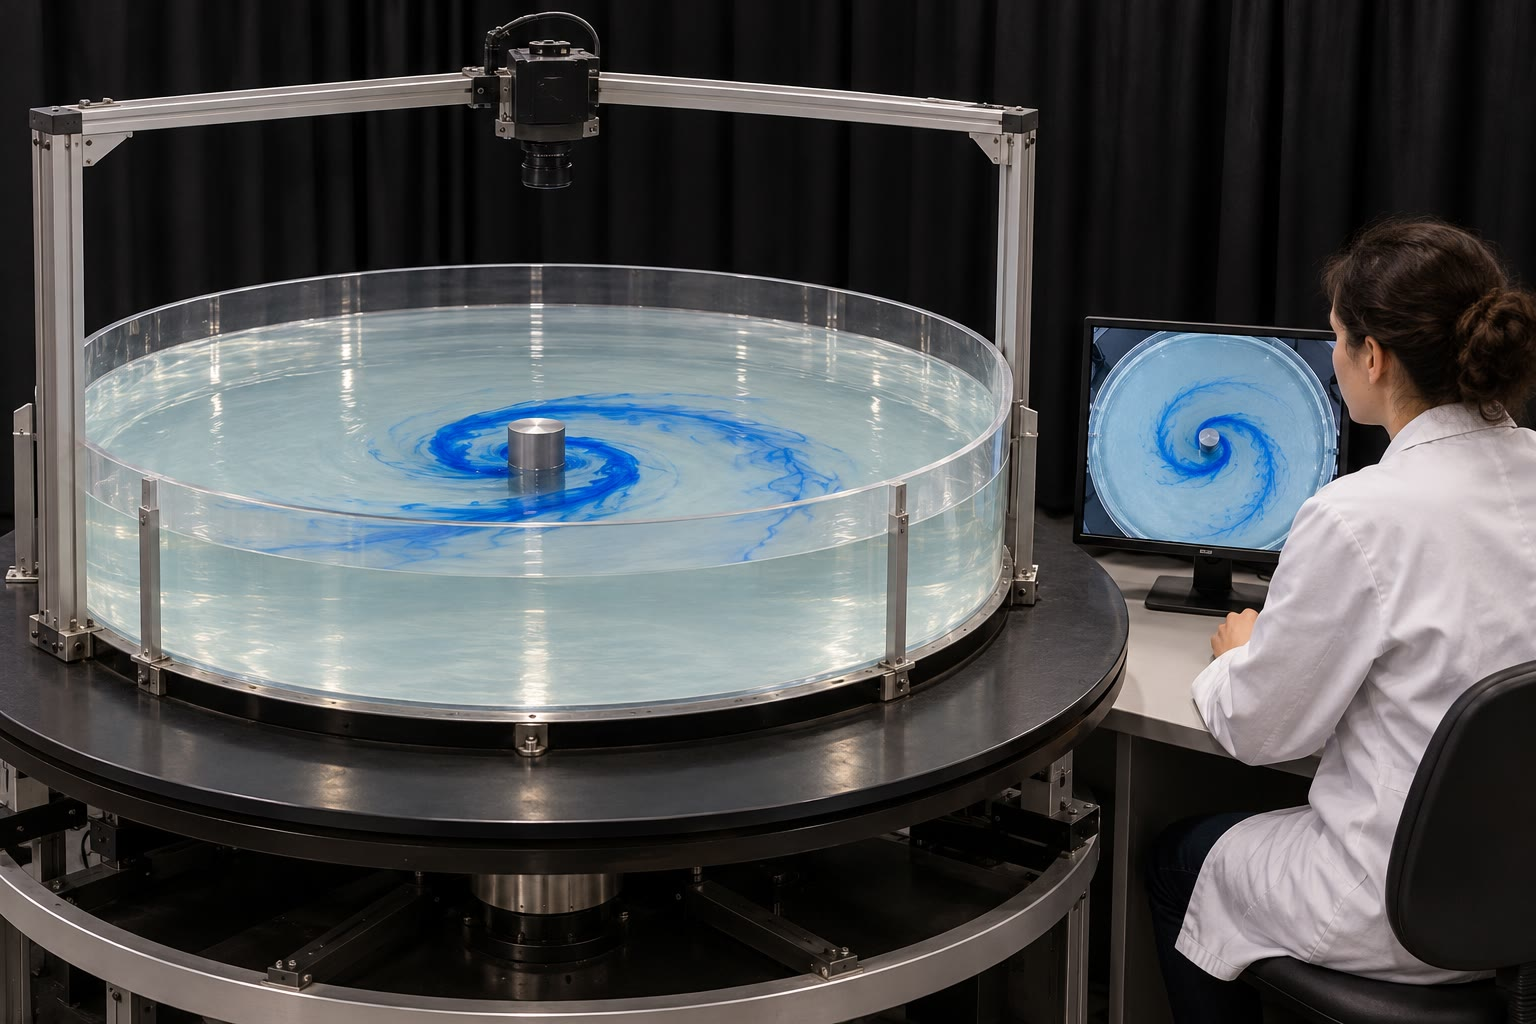
\includegraphics[width=\linewidth]{images/book5/ai/b3-rotating-tank.jpg}

{\scriptsize 旋转水箱：染料绕圆柱螺旋上升，由
随转盘转动的照相机拍摄（AI 生成的插图）。}
\end{minipage}
\end{inthelab}

\section{练习}

\begin{exercise}[$\star$]\label{exo:b3:gfd-foundations:1}
取 $\Omega = \qty{7.292115e-5}{rad/s}$。(a)~求北纬
\ang{30}、\ang{45} 和 \ang{60} 处的科里奥利参数与惯性周期。
(b)~求速度为
\qty{0.20}{m/s} 的洋流在相同纬度处的惯性圆半径。(c)~将北纬
\ang{30} 处的惯性周期与恒星日 \qty{23.9345}{h} 比较。
\end{exercise}

\begin{exercise}[$\star$]\label{exo:b3:gfd-foundations:2}
求北纬 \ang{45} 处以下各系统的\omterm{def:b3:gfd-foundations:numbers}{罗斯贝数}：尘卷风（\qty{10}{m/s}，
\qty{10}{m}）、海风（\qty{5}{m/s}，\qty{20}{km}）、低压
（\qty{15}{m/s}，\qty{1000}{km}）和海洋环流（\qty{0.05}{m/s}，
\qty{2000}{km}）。其中哪些接近地转平衡？
\end{exercise}

\begin{exercise}[$\star$]\label{exo:b3:gfd-foundations:3}
北纬 \ang{45} 处对流层的平均温度为 \qty{250}{K}，
每向北 \qty{1000}{km} 下降 \qty{5}{K}。利用\omterm{thm:b3:gfd-foundations:thermal-wind}{热成风}在高度方向上的第一项，
求西风的竖直切变，
以及风速在 \qty{10}{km} 内的增量。
\end{exercise}

\begin{exercise}[$\star$]\label{exo:b3:gfd-foundations:4}
海洋上层一千米内的稳定度 $E = -(1/\rho)\,\mathrm d\rho_\theta/\mathrm dz$
介于 \num{50e-8} 与 \qty{1000e-8}{m^{-1}} 之间；在深海海沟中为 \qty{e-8}{m^{-1}}。
对下列三个取值，计算 $N = \sqrt{gE}$、
浮力振荡的周期，
以及以每小时周数表示的 $N$。
\end{exercise}

\begin{exercise}[$\star\star$]\label{exo:b3:gfd-foundations:5}
某天气系统的 $U = \qty{10}{m/s}$，$L = \qty{1000}{km}$，$H =
\qty{10}{km}$，位于北纬 \ang{45}。(a)~估算其竖直速度与竖直加速度，
并将后者与 $g$ 及气压扰动的竖直梯度 $fUL/H$ 比较。(b)~求被舍去的
科里奥利项 $\tilde fu$，
并与 $g$ 比较。
\end{exercise}

\begin{exercise}[$\star\star$]\label{exo:b3:gfd-foundations:6}
取 $f = \qty{e-4}{s^{-1}}$，圆形等压线半径为
\qty{300}{km}。(a)~低压周围的气压梯度给出 $V_g =
\qty{20}{m/s}$，求\omterm{def:b3:gfd-foundations:gradient}{梯度风}。(b)~高压周围，
$V_g = \qty{5}{m/s}$，求\omterm{def:b3:gfd-foundations:gradient}{梯度风}。(c)~高压周围，
$V_g$ 可能的最大值是多少？此时的风速如何？
\end{exercise}

\begin{exercise}[$\star\star$]\label{exo:b3:gfd-foundations:7}
水箱深 \qty{20}{cm}，每 \qty{6}{s} 转一圈；水的运动黏度 $\nu =
\qty{e-6}{m^2/s}$。(a)~求 $f = 2\Omega$，再求速度为 \qty{1}{cm/s} 的水流
流过直径为 \qty{5}{cm} 的圆柱时的\omterm{def:b3:gfd-foundations:numbers}{罗斯贝数}，以及水箱的\omterm{def:b3:gfd-foundations:numbers}{埃克曼数}。
是否会形成\omterm{thm:b3:gfd-foundations:taylor-proudman}{泰勒柱}？(b)~理论给出起转时间 $H/\sqrt{\nu\Omega}$，
求其值，分别以分钟和转盘转数表示。
\end{exercise}

\begin{exercise}[$\star\star$]\label{exo:b3:gfd-foundations:8}
在 1991--2020 年一月的纬向平均中，北纬 \ang{30} 处的西风
在 \qty{850}{hPa} 处为 \qty{4.27}{m/s}，在 \qty{250}{hPa} 处为 \qty{40.39}{m/s}；
北纬 \ang{45} 处分别为 \qty{5.99}{m/s} 和 \qty{23.17}{m/s}。取 $R =
\qty{286.9}{J.kg^{-1}.K^{-1}}$，求两个纬度处层平均温度的经向梯度，
并说明为何急流在
北纬 \ang{30} 处更强。
\end{exercise}

\begin{exercise}[$\star\star$]\label{exo:b3:gfd-foundations:9}
(a)~求对流层的\omterm{def:b3:gfd-foundations:rossby-radius}{罗斯贝变形半径}（$N =
\qty{0.0113}{s^{-1}}$，$H = \qty{11}{km}$，北纬 \ang{45}）以及
上层海洋的\omterm{def:b3:gfd-foundations:rossby-radius}{罗斯贝变形半径}（$N = \qty{0.00357}{s^{-1}}$，$H = \qty{1000}{m}$，北纬 \ang{40.5}）。
(b)~取 $a = \qty{6371}{km}$，求两个纬度处的 $\beta$，以及
科里奥利参数在每个半径上的相对变化 $\beta L_R/f$。
\end{exercise}

\begin{exercise}[$\star\star\star$]\label{exo:b3:gfd-foundations:10}
表层海洋中一个以速度 $U$ 运动的水团受线性
摩擦减速：$\mathrm du/\mathrm dt = fv - ru$，$\mathrm dv/\mathrm dt = -fu -
rv$。(a)~令 $w = u + \mathrm iv$ 求解，并描述其路径。(b)~该水团还受一股稳定的
向东洋流 $u_0$ 携带，求其位置。
(c)~在北纬 \ang{45}，取 $U = \qty{0.2}{m/s}$，$r^{-1} =
\num{4}\text{ 天}$，$u_0 = \qty{0.05}{m/s}$，求四天后其相对洋流的速率，
以及它漂移的距离。
\end{exercise}

\begin{exercise}[$\star\star\star$]\label{exo:b3:gfd-foundations:11}
穿过北纬 \ang{40} 处的海洋锋面，水的密度向北增加，
在上层 \qty{1000}{m} 内，每 \qty{100}{km} 增加 \qty{1}{kg/m^3}；
其下的水则均匀且静止。取 $\rho_0 =
\qty{1025}{kg/m^3}$，求洋流的竖直切变，
以及表面的洋流。洋流朝哪个方向流动？
\end{exercise}

\begin{exercise}[$\star\star\star$]\label{exo:b3:gfd-foundations:12}
位于 北纬 \ang{40.5}、西经 \ang{30.5} 处的年平均水柱，其\omterm{def:b3:gravity-geodesy:geopotential}{位势}
密度 $\sigma_\theta = \rho_\theta - \qty{1000}{kg/m^3}$ 在表层为 26.029，
在 \qty{100}{m} 处为 26.697，在 \qty{500}{m} 处为 27.079，在
\qty{1000}{m} 处为 27.628。(a)~计算三层各自的 $N$，
分别以 \unit{s^{-1}} 和每小时周数表示。(b)~哪一层最稳定，
原因何在？(c)~将所得数值与
\cref{exo:b3:gfd-foundations:4}中上层海洋的范围进行比较。
\end{exercise}
% ledger: geod5:grs80-defining, earth:Trot, stewart:stability, data:b5-ncep-uwnd, data:b5-woa23-atlantic, earth:Rmean

\section{问题：奥林草原上的风}

\begin{problem}[{周末问题——旋转、层结与
位于北纬 \ang{48} 的虚构平原上的风}]
\label{pb:b3:gfd-foundations:1}
奥林草原是一片平坦的平原，位于 北纬 \ang{48}，上有奥林湖，
湖宽 \qty{12}{km}，另有一间配备旋转水槽的小型实验室。取
$\Omega = \qty{7.292115e-5}{rad/s}$, $g = \qty{9.81}{m/s^2}$, $R =
\qty{286.9}{J.kg^{-1}.K^{-1}}$ 和 $c_p = \qty{1004}{J.kg^{-1}.K^{-1}}$。
草原、湖泊及其风的所有数值均为虚构。

\medskip\noindent\textbf{第一部分——旋转是否重要？}
\begin{enumerate}
\item 计算奥林草原处的科里奥利参数和惯性周期。
\item 计算下列五种流动的\omterm{def:b3:gfd-foundations:numbers}{罗斯贝数}：从浴缸中排出的水
  （速度 \qty{0.1}{m/s}，尺度 \qty{0.3}{m}）；实验室的水槽，每
  \qty{10}{s} 转一圈（取 $f = 2\Omega_{\text{水槽}}$；速度 \qty{5}{mm/s}，
  尺度 \qty{0.2}{m}）；傍晚的湖风（\qty{5}{m/s}，
  \qty{20}{km}）；低压（\qty{15}{m/s}，\qty{1000}{km}）；同一纬度的
  大洋盆地环流（\qty{0.05}{m/s}，\qty{2000}{km}）。
\item 其中哪些流动能感受到驱动它们的旋转，
  哪些接近地转？
\item 计算水槽（深度 \qty{0.2}{m}，$\nu =
  \qty{e-6}{m^2/s}$），低压（涡动黏度 \qty{10}{m^2/s}，
  深度 \qty{10}{km}），以及环流（涡动黏度 \qty{e-3}{m^2/s}，
  深度 \qty{1000}{m}）的\omterm{def:b3:gfd-foundations:numbers}{埃克曼数}。
\item 埃克曼层的厚度为 $\delta = \sqrt{2\nu/f}$。证明
  $\delta/H = \sqrt{2\,\mathrm{Ek}}$，并计算水槽及
  奥林草原上空气的 $\delta$。
\item 这些数值说明摩擦在何处起重要作用？
\end{enumerate}

\medskip\noindent\textbf{第二部分——近地面的风。}
\begin{enumerate}[resume]
\item 地面气压为 \qty{1012.9}{hPa}，气温为
  \qty{288.1}{K}。计算空气的密度。
\item 海平面气压向北每
  \qty{300}{km} 下降 \qty{4}{hPa}。计算地转风并给出其方向。
\item 同样的气压梯度环绕一个低压，其等压线半径为
  \qty{600}{km}。计算等压线的\omterm{def:b3:gfd-foundations:numbers}{罗斯贝数}和
  \omterm{def:b3:gfd-foundations:gradient}{梯度风}。
\item 同样的气压梯度环绕一个半径相同的反气旋。
  计算\omterm{def:b3:gfd-foundations:gradient}{梯度风}，以及该反气旋能维持的最大气压梯度（以
  \unit{hPa} 每 \qty{300}{km} 计）。
\end{enumerate}

\medskip\noindent\textbf{第三部分——层结。}
\begin{enumerate}[resume]
\item 对流层气温以 \qty{6.49}{K/km} 的速率下降。
  计算干绝热递减率 $g/c_p$，以及 \qty{5}{km} 处的 $N$ 和
  浮力振荡周期（该处气温为
  \qty{255.7}{K}）。
\item 在 \qty{11}{km} 以上，空气为等温的，温度为 \qty{216.6}{K}。证明
  该处 $N^2 = g^2/(c_pT)$，并计算 $N$ 及其与
  第 11 题中数值的比值。
\item 计算奥林草原上空对流层的\omterm{def:b3:gfd-foundations:rossby-radius}{罗斯贝变形半径}，所用的 $N$ 取自
  第 11 题，$H = \qty{10}{km}$，并将其与第一部分中
  低压的尺度作比较。
\item 夏季，奥林湖上层 \qty{20}{m} 的水比深层水轻
  \qty{1.5}{kg/m^3}（$\rho_0 = \qty{1000}{kg/m^3}$）。计算
  约化重力 $g' = g\,\Delta\rho/\rho_0$，上层慢内波的
  速度 $\sqrt{g'h}$，以及\omterm{def:b3:gfd-foundations:rossby-radius}{罗斯贝变形半径}
  $\sqrt{g'h}/f$。
\item 地球自转是否会影响湖泊内部的运动？
\end{enumerate}

\medskip\noindent\textbf{第四部分——\omterm{thm:b3:gfd-foundations:thermal-wind}{热成风}。}
\begin{enumerate}[resume]
\item 两座探空站位于同一经线上，相距 \qty{600}{km}。
  从地面（\qty{1013}{hPa}）至
  \qty{265}{hPa}（约 \qty{10}{km}）这一层的平均气温，南站为 \qty{253.0}{K}，
  北站为 \qty{249.4}{K}。计算
  气温的经向梯度，单位取 \unit{K} 每 \qty{1000}{km}。
\item 两气压之间的层厚为 $\Delta z = (R\bar
  T/g)\ln(p_b/p_t)$。计算两站的层厚，以及
  \qty{265}{hPa} 等压面相对于地面等压面的斜率。
\item 由该斜率推出地转风从地面至
  \qty{265}{hPa} 的增量。
\item 用压力坐标下的\omterm{thm:b3:gfd-foundations:thermal-wind}{热成风}定理计算同一增量。
\item 奥林草原的空气是正压的还是\omterm{def:b3:gfd-foundations:baroclinic}{斜压}的？若是正压，
  则 \qty{265}{hPa} 处的风会是多少？
\item 用\omterm{thm:b3:gfd-foundations:thermal-wind}{热成风}的第一项计算高度坐标下的增量，
  取标准对流层在 0 至
  \qty{10}{km} 之间的平均气温 \qty{255.7}{K}，并进行比较。
\item 计算 \qty{541}{hPa}（约 \qty{5}{km}）处的风，假设
  各层的气温梯度相同。
\item 理查森数 $N^2/(\partial u/\partial z)^2$ 须降到
  0.25 以下，切变才能驱动湍流。计算奥林草原上空对流层的
  理查森数。
\item 一月份，\qty{250}{hPa} 处的纬向平均西风，在
北纬 \ang{45} 处为 \qty{23.2}{m/s}，在 北纬 \ang{30} 处为 \qty{40.4}{m/s}。
  将其与奥林草原的风相比较，并解释为何局地风可以超过纬向平均值。
\item 给出奥林草原上空 \qty{10}{km} 处的地转风。
\end{enumerate}
\end{problem}
% ledger: geod5:grs80-defining, stewart:stability, data:b5-ncep-uwnd, nasa:grc-atmos
